\documentclass[a4paper, 12pt]{article}
\usepackage{blindtext}
\usepackage[margin=2 cm]{geometry}
\usepackage[spanish]{babel}
\usepackage[utf8]{inputenc}
\usepackage{array}
\usepackage{amsmath}
\usepackage{graphicx}
\usepackage{ifthen}
\usepackage{commath}
\usepackage{esint}
\usepackage{mathtools}
\usepackage{listing}
\usepackage{multirow}
\usepackage{tabto}
\usepackage[backend=biber]{biblatex}
\usepackage{csquotes}
\usepackage{float}
\usepackage{amssymb}
\usepackage{physics}
\usepackage{hyperref}
\usepackage[shortlabels]{enumitem}
\selectlanguage{spanish}
\decimalpoint

\begin{document}
    \begin{center}
        \begin{Large}

            \begin{figure}[H]	
                \centering
                
\includegraphics[width = 6cm]{./img/logo_UADY.png}
                \label{uady}
            \end{figure}
            \textsc{FACULTAD DE INGENIERÍA}
                
            \medskip

            Curso Agosto - Diciembre 2021

            \medskip

            \textsc{Física Computacional}

            \medskip

            \textsl{Actividad de Aprendizaje 1}

            \medskip

            Br. Alejandro Santoscoy Rivero

            \medskip

            Dr. Francisco Ramón Peñuñuri Anguiano

            \rule{0.3\paperwidth}{0.5pt}

            \medskip

            27 de Septiembre de 2021

        \end{Large}
    \end{center}
    \pagenumbering{roman}
    \newpage
    \pagenumbering{arabic}

    \section{Problema}

    Considere el mecanismo planar $4R$ de la Figura \ref{Figura:1}. Haga una propagación de errores por Monte Carlo, en los parámetros $r_k (k = 1, 2, 3, 4, c_x, c_y)$ para la trayectoria generada por el punto $r_\text{gen}$. Tome como ángulos de entrada 10 puntos aleatorios en $[0, 2\pi)$. Como parámetros del mecanismo use los valores que se muestran en el Cuadro \ref{Tabla:1}. Suponga que las cantidades están en el sistema internacional de unidades y considere $\Delta r_k = 10^{-5} \text{m}$.

    Para la simulación use 100 realizaciones probabilísticas.

    \begin{table}[h!]
        \centering
        \begin{tabular}{ c c c c c c c c c }
            \hline
            $x_0$ & $y_0$ & $r_1$ & $r_2$ & $r_3$ & $r_4$ & $r_{cx}$ & $r_{cy}$ & $\theta_0$ \\
            \hline
            0.00000 & 0.00000 & 1.08913 & 0.42259 & 0.964444 & 0.58781 & 0.39137 & 0.42950 & 0.00000 \\
            \hline
        \end{tabular}
        \caption{Parámetros del mecanismo}
        \label{Tabla:1}
    \end{table}

    \begin{figure}[h]
        \centering
        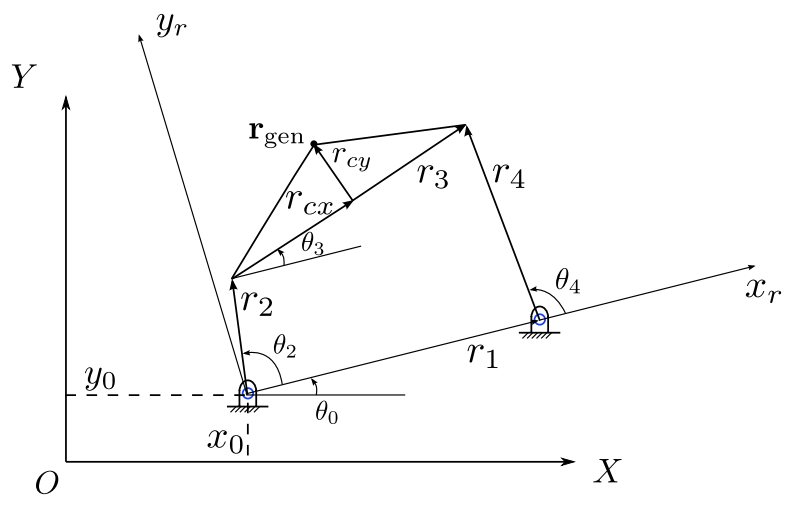
\includegraphics[width=12cm]{img/mecanismo.png}
        \caption{Mecanismo 4R planar}
        \label{Figura:1}
    \end{figure}

    Definiendo

    \begin{align*}
        l_1 &= r_1 / r_2, \\
        l_2 &= r_1 / r_3, \\
        l_3 &= \qty( r_4^2 - r_1^2 - r_2^2 - r_3^2 ) / \qty(2r_2 r_3), \\
        k_a &= \cos \theta_2 - l_1 + l_2 \cos \theta_2 + l_3, \\
        k_b &= -2 \sin \theta_2, \\
        k_c &= l_1 + \qty(l_2 - 1) \cos \theta_2 + l_3
    \end{align*}

    las coordenadas del punto

    \begin{equation*}
        r_\text{gen} \qty(\theta_2; x_0, y_0, r_1, r_2, r_3, r_4, r_{cx}, r_{cy}, \theta_0) = \qty(P_x, P_y),
    \end{equation*}

    están dadas por

    \begin{align*}
        P_x &= x_0 + r_2 \cos \qty(\theta_2 + \theta_0) + r_{cx} \cos \qty(\theta_3 + \theta_0) - r_{cy} \sin \qty(\theta_3 + \theta_0) \\
        P_y &= y_0 + r_2 \sin \qty(\theta_2 + \theta_0) + r_{cx} \sin \qty(\theta_3 + \theta_0) - r_{cy} \cos \qty(\theta_3 + \theta_0), \\
    \end{align*}

    con $\theta_3$ dado por

    \begin{equation*}
        \theta_3 = 2 \text{atan}2 \qty(-k_b - \sqrt{k_b^2 - 4 k_a k_c}, 2k_a).
    \end{equation*}

    \section{Resolución}

    Se utiliza el software de Octave como apoyo en la simulación del proceso, esto debido a su capacidad de manipulación matricial.

    La resolución será explicada junto con el código para tener una comprensión más directa y exacta de lo que sucede.

    Se comienza con el formato en consola, limpiando todas las variables y limpiando la salida.

    \begin{verbatim}
        clc;
        clear all;
        format long;
    \end{verbatim}

    Se define una función que genera cierta cantidad de números aleatorios dentro de una rango específico.

    \begin{verbatim}
        function local = X0(m,bL,bU)
            n = size(bL,2);
            local = zeros(m,n);
            for i = 1:m
                for j = 1:n
                    local(i,j) = bL(j) + (bU(j) - bL(j))*rand();
                endfor
            endfor
        end
    \end{verbatim}

    Se inicializan los parámetros del mecanismo.

    \begin{verbatim}
        x0      = 0.00000;
        y0      = 0.00000;
        r1      = 1.08913;
        r2      = 0.42255;
        r3      = 0.96444;
        r4      = 0.58781;
        rcx     = 0.39137;
        rcy     = 0.42950;
        theta0  = 0.00000;
    \end{verbatim}

    Se generan 10 ángulos aleatorios entre $0$ y $2\pi$ tanto para las variables \verb|theta2| y \verb|theta4|.

    \begin{verbatim}
        theta2  = X0(10,0,2*pi);
        theta4  = X0(10,0,2*pi);
    \end{verbatim}

    Se define la discrepancia $\Delta r_k$ como

    \begin{verbatim}
        delta = 0.00001;
    \end{verbatim}

    Se generan 100 mediciones aleatorias de cada barra dentro del rango de discrepancia definido.

    \begin{verbatim}
        r1_rand  = X0(100, r1-delta, r1+delta);
        r2_rand  = X0(100, r2-delta, r2+delta);
        r3_rand  = X0(100, r3-delta, r3+delta);
        r4_rand  = X0(100, r4-delta, r4+delta);
        rcx_rand = X0(100, rcx-delta, rcx+delta);
        rcy_rand = X0(100, rcy-delta, rcy+delta);
    \end{verbatim}

    De estas medidas se obtienen los siguientes parámetros.

    \begin{verbatim}
        l1 = r1_rand./r2_rand;
        l2 = r1_rand./r3_rand;
        l3 = (r4_rand.^2-r1_rand.^2-r2_rand.^2-r3_rand.^2)/(2*r2.*r3);
    \end{verbatim}

    Ahora la lógica implementada es realizar 10 mediciones, una por cada valor del ángulo, el resultado de esto es obtener 10 puntos de los cuales se conocerán su promedio y desviación estándar en $x$ y $y$. (Se agregan saltos de línea en las expresiones \verb|rgenx| y \verb|rgeny| para facilitar la lectura, pero la sintaxis debe escribirse en una sola línea).

    \begin{verbatim}
        for ii = 1:size(theta2)(1)
            ka(:,ii) = cos(theta2)(ii) - l1  + l2 .* cos(theta2)(ii) + l3;
            kb(:,ii) = -2*sin(theta2)(ii);
            kc(:,ii) = l1 + (l2-1) .* cos(theta2)(ii) + l3;

            theta3 = 2*atan2(-kb-sqrt(kb.^2-4*ka.*kc),2*ka);
            
            rgenx(:,ii) = x0 +
                          r2_rand*cos(theta2(ii)+theta0) +
                          rcx_rand.*cos(theta3(:,ii)-theta0) -
                          rcy_rand.*sin(theta3(:,ii)-theta0);

            rgeny(:,ii) = y0 +
                          r2_rand*sin(theta2(ii)+theta0) +
                          rcx_rand.*sin(theta3(:,ii)-theta0) +
                          rcy_rand.*cos(theta3(:,ii)-theta0);
            
            rgenx_avg(ii) = mean(rgenx(:,ii));
            rgeny_avg(ii) = mean(rgeny(:,ii));
            
            rgenx_std(ii) = std(rgenx(:,ii));
            rgeny_std(ii) = std(rgeny(:,ii));
        endfor
    \end{verbatim}

    Y por último mostrar los datos obtenidos en una misma gráfica representando la localización del promedio y de la desviación estándar.

    \begin{verbatim}
        clf;
        hold on;
        scatter(rgenx_avg, rgeny_avg, 15, 'r');
        scatter(rgenx_avg+rgenx_std, rgeny_avg, 5, 'b');
        scatter(rgenx_avg-rgenx_std, rgeny_avg, 5, 'b');
        scatter(rgenx_avg, rgeny_avg+rgeny_std, 5, 'b');
        scatter(rgenx_avg, rgeny_avg-rgeny_std, 5, 'b');
        hold off;
    \end{verbatim}

    Los resultados se resumen en la descripción de las variables: $\theta_2$, $\langle x \rangle$, $\langle y \rangle$, $\sigma_x$ y $\sigma_y$. Al tener 10 ángulos aleatorios, los 10 resultados obtenidos se pueden apreciar en la Tabla \ref{Tabla:2}.

    \begin{table}[h!]
        \centering
        \begin{tabular}{|c|c|c|c|c|}
            \hline
            $\theta_2$ & $\langle x \rangle$ & $\langle y \rangle$ & $\sigma_x$ & $\sigma_y$ \\
            \hline
            1.173308006 & 0.45847392 & 0.890280486 & 1.96E-05 & 7.12E-06 \\
            4.187756579 & -0.168292212 & 0.21372828 & 1.59E-05 & 7.68E-06 \\
            6.223366105 & 0.455343172 & 0.55483861 & 3.01E-05 & 5.60E-06 \\
            4.995621966 & -2.12E-02 & 0.158423949 & 1.50E-05 & 6.53E-06 \\
            4.55679268 & -0.121014098 & 0.160963874 & 1.45E-05 & 6.79E-06 \\
            4.452553013 & -0.138038859 & 0.171954797 & 1.47E-05 & 6.95E-06 \\
            5.833120384 & 0.282741983 & 0.388972114 & 2.39E-05 & 6.32E-06 \\
            5.604391827 & 0.184880522 & 0.297642549 & 2.01E-05 & 6.56E-06 \\
            4.803157512 & -7.03E-02 & 0.15002794 & 1.45E-05 & 6.59E-06 \\
            1.574956807 & 0.318644318 & 0.907298553 & 1.66E-05 & 7.06E-06 \\
            \hline
        \end{tabular}
        \caption{Parámetros del mecanismo}
        \label{Tabla:2}
    \end{table}

    La distribución de cada uno de los 10 puntos se puede ver en la Figura \ref{GraficaGeneral}.

    \begin{figure}[h!]
        \centering
        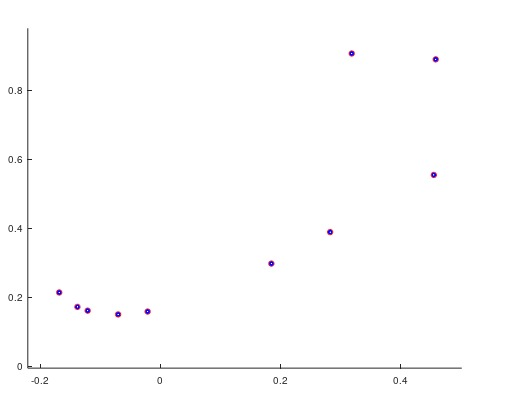
\includegraphics[width=12cm]{img/graficaPuntos.jpeg}
        \caption{Gráfica de los 10 puntos medidos con distinto ángulo}
        \label{GraficaGeneral}
    \end{figure}

    Y la visualización de cada punto promedio junto con sus respectivas desviaciones estándar en $x$ y $y$ se ven entre la Figura \ref{G1} y la Figura \ref{G10}.

    El código se puede encontrar en el siguiente repositorio de GitHub: \url{https://github.com/Santocoyo/ComputationalPhysics_Task1}

    \begin{figure}[ht!]
        \centering
        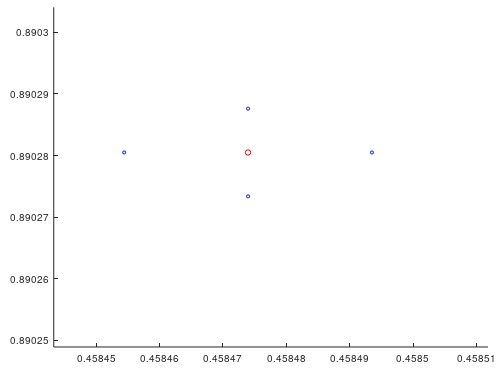
\includegraphics[width=12cm]{img/g1.jpeg}
        \caption{Gráfica del promedio y desviación estándar con un ángulo de 1.17 rad}
        \label{G1}
    \end{figure}

    \begin{figure}[ht!]
        \centering
        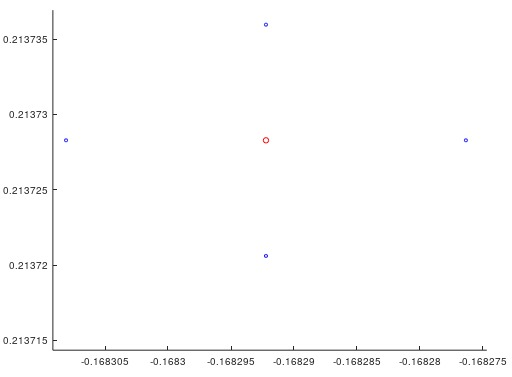
\includegraphics[width=12cm]{img/g2.jpeg}
        \caption{Gráfica del promedio y desviación estándar con un ángulo de 4.18 rad}
        \label{G2}
    \end{figure}

    \begin{figure}[ht!]
        \centering
        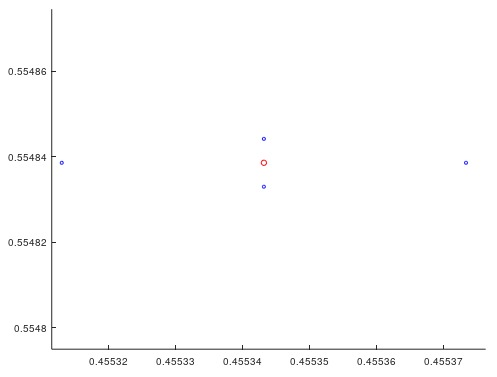
\includegraphics[width=12cm]{img/g3.jpeg}
        \caption{Gráfica del promedio y desviación estándar con un ángulo de 6.22 rad}
        \label{G3}
    \end{figure}

    \begin{figure}[ht!]
        \centering
        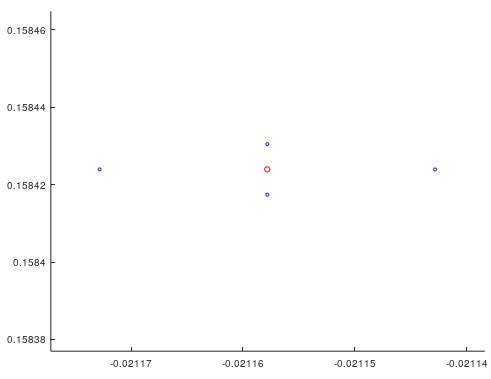
\includegraphics[width=12cm]{img/g4.jpeg}
        \caption{Gráfica del promedio y desviación estándar con un ángulo de 4.99 rad}
        \label{G4}
    \end{figure}

    \begin{figure}[ht!]
        \centering
        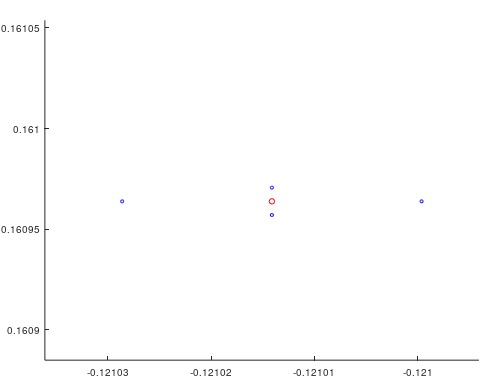
\includegraphics[width=12cm]{img/g5.jpeg}
        \caption{Gráfica del promedio y desviación estándar con un ángulo de 4.55 rad}
        \label{G5}
    \end{figure}

    \begin{figure}[ht!]
        \centering
        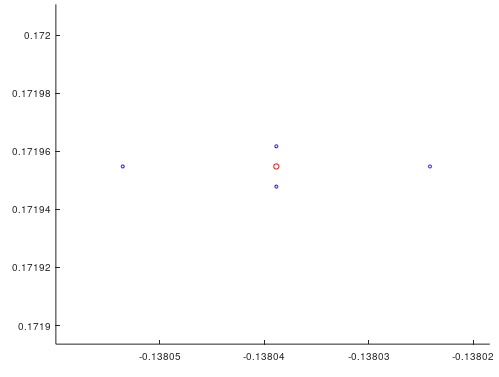
\includegraphics[width=12cm]{img/g6.jpeg}
        \caption{Gráfica del promedio y desviación estándar con un ángulo de 4.45 rad}
        \label{G6}
    \end{figure}

    \begin{figure}[ht!]
        \centering
        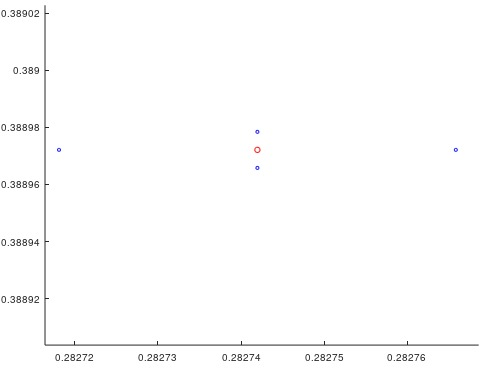
\includegraphics[width=12cm]{img/g7.jpeg}
        \caption{Gráfica del promedio y desviación estándar con un ángulo de 5.83 rad}
        \label{G7}
    \end{figure}

    \begin{figure}[ht!]
        \centering
        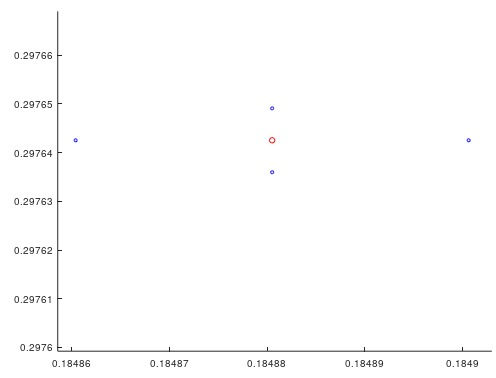
\includegraphics[width=12cm]{img/g8.jpeg}
        \caption{Gráfica del promedio y desviación estándar con un ángulo de 5.60 rad}
        \label{G8}
    \end{figure}

    \begin{figure}[ht!]
        \centering
        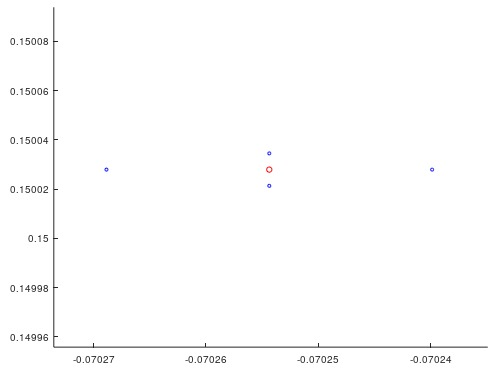
\includegraphics[width=12cm]{img/g9.jpeg}
        \caption{Gráfica del promedio y desviación estándar con un ángulo de 4.80 rad}
        \label{G9}
    \end{figure}

    \begin{figure}[ht!]
        \centering
        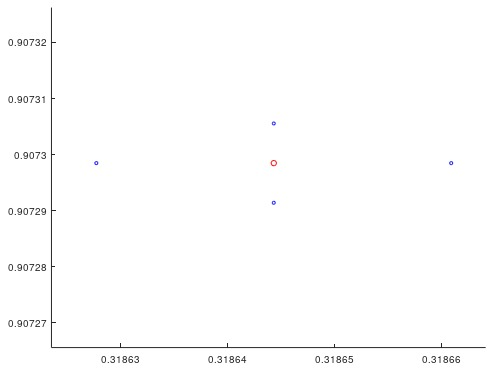
\includegraphics[width=12cm]{img/g10.jpeg}
        \caption{Gráfica del promedio y desviación estándar con un ángulo de 1.57 rad}
        \label{G10}
    \end{figure}

\end{document}